
\documentclass[10pt,a4paper]{article}
\usepackage[T1]{fontenc}
\usepackage{tikz}
\usepackage[margin=1cm]{geometry}
\begin{document}

% Explanation about the algorithm
\section*{Binary Tree Deletion Algorithm}
In this document, we illustrate the deletion process of a binary tree. The algorithm used for deleting a node involves the following steps:

\begin{itemize}
    \item \textbf{Finding the Node:} We first perform a level-order traversal (breadth-first search) to locate the node to be deleted and the deepest node in the tree.
    \item \textbf{Replacing Data:} We replace the data of the node to be deleted with the data of the deepest node.
    \item \textbf{Deleting Deepest Node:} We then delete the deepest node from the tree.
\end{itemize}

\section*{Deletion Steps}
The following figures illustrate the binary tree at various steps of the deletion process.


\begin{figure}[h!]
\centering

\begin{minipage}{0.8\textwidth}
    \centering
    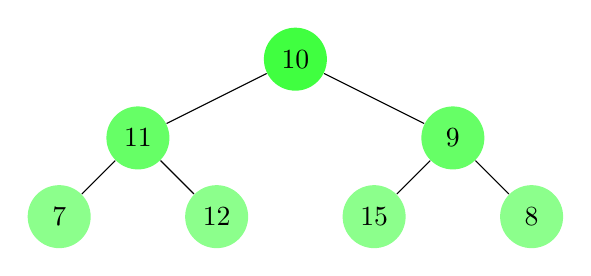
\begin{tikzpicture}[level distance=10mm]
        \tikzstyle{every node}=[fill=green!75,circle,inner sep=1pt, minimum size=8mm]
        \tikzstyle{level 1}=[sibling distance=40mm, set style={{every node}+=[fill=green!60]}]
        \tikzstyle{level 2}=[sibling distance=20mm, set style={{every node}+=[fill=green!45]}]
        \tikzstyle{level 3}=[sibling distance=15mm, set style={{every node}+=[fill=green!30]}]
        \tikzstyle{level 4}=[sibling distance=10mm, set style={{every node}+=[fill=green!15]}]
        \node {10} child {node {11} child {node {7} } child {node {12} }} child {node {9} child {node {15} } child {node {8} }};
    \end{tikzpicture}
    \caption{Step 1 (Initial tree)}
\end{minipage}
\vspace{1cm}

\begin{minipage}{0.8\textwidth}
    \centering
    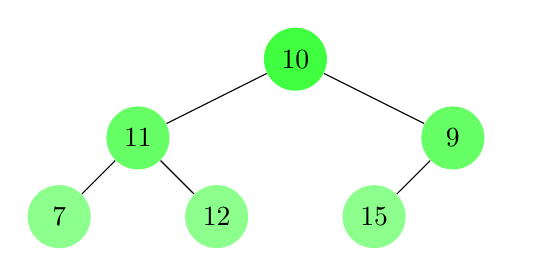
\begin{tikzpicture}[level distance=10mm]
        \tikzstyle{every node}=[fill=green!75,circle,inner sep=1pt, minimum size=8mm]
        \tikzstyle{level 1}=[sibling distance=40mm, set style={{every node}+=[fill=green!60]}]
        \tikzstyle{level 2}=[sibling distance=20mm, set style={{every node}+=[fill=green!45]}]
        \tikzstyle{level 3}=[sibling distance=15mm, set style={{every node}+=[fill=green!30]}]
        \tikzstyle{level 4}=[sibling distance=10mm, set style={{every node}+=[fill=green!15]}]
        \node {10} child {node {11} child {node {7} } child {node {12} }} child {node {9} child {node {15} } child[fill=none] {edge from parent[draw=none]}};
    \end{tikzpicture}
    \caption{Step 2}
\end{minipage}
\vspace{1cm}

\begin{minipage}{0.8\textwidth}
    \centering
    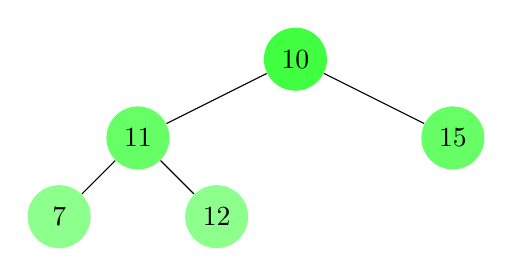
\begin{tikzpicture}[level distance=10mm]
        \tikzstyle{every node}=[fill=green!75,circle,inner sep=1pt, minimum size=8mm]
        \tikzstyle{level 1}=[sibling distance=40mm, set style={{every node}+=[fill=green!60]}]
        \tikzstyle{level 2}=[sibling distance=20mm, set style={{every node}+=[fill=green!45]}]
        \tikzstyle{level 3}=[sibling distance=15mm, set style={{every node}+=[fill=green!30]}]
        \tikzstyle{level 4}=[sibling distance=10mm, set style={{every node}+=[fill=green!15]}]
        \node {10} child {node {11} child {node {7} } child {node {12} }} child {node {15} };
    \end{tikzpicture}
    \caption{Step 3}
\end{minipage}
\vspace{1cm}

\begin{minipage}{0.8\textwidth}
    \centering
    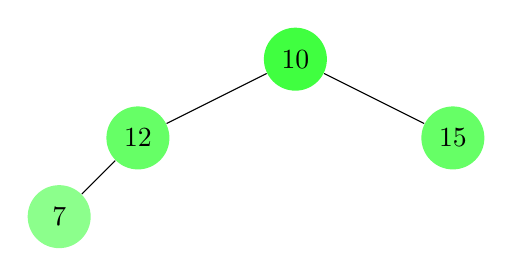
\begin{tikzpicture}[level distance=10mm]
        \tikzstyle{every node}=[fill=green!75,circle,inner sep=1pt, minimum size=8mm]
        \tikzstyle{level 1}=[sibling distance=40mm, set style={{every node}+=[fill=green!60]}]
        \tikzstyle{level 2}=[sibling distance=20mm, set style={{every node}+=[fill=green!45]}]
        \tikzstyle{level 3}=[sibling distance=15mm, set style={{every node}+=[fill=green!30]}]
        \tikzstyle{level 4}=[sibling distance=10mm, set style={{every node}+=[fill=green!15]}]
        \node {10} child {node {12} child {node {7} } child[fill=none] {edge from parent[draw=none]}} child {node {15} };
    \end{tikzpicture}
    \caption{Step 4}
\end{minipage}
\vspace{1cm}

\end{figure}
\newpage

\end{document}
